\documentclass[crop]{standalone}
\usepackage{pgfplots}
\begin{document}
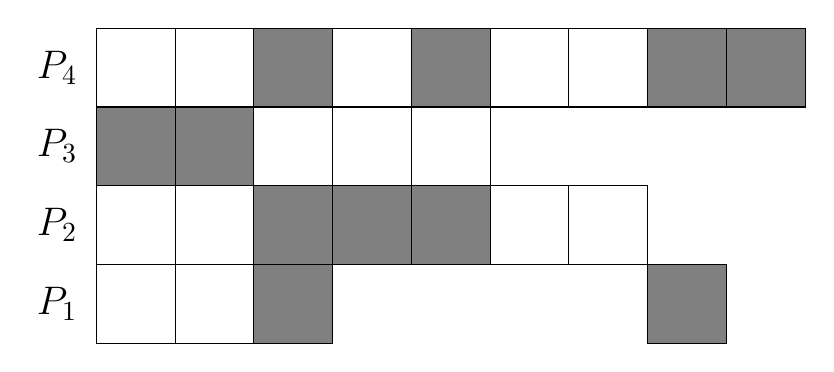
\begin{tikzpicture}
\def\y{1}
\node at (0,\y) {\Large \(P_{1}\)};
\foreach \x in {1,2} {
\node[draw, rectangle, fill=none, inner sep=0.5cm] at (\x, \y) {};
}
\foreach \x in {3,8} {
\node[draw, rectangle, fill=gray, inner sep=0.5cm] at (\x, \y) {};
}

\def\y{2}
\node at (0,\y) {\Large \(P_{2}\)};
\foreach \x in {1,2,6,7} {
\node[draw, rectangle, fill=none, inner sep=0.5cm] at (\x, \y) {};
}
\foreach \x in {3,4,5} {
\node[draw, rectangle, fill=gray, inner sep=0.5cm] at (\x, \y) {};
}

\def\y{3}
\node at (0,\y) {\Large \(P_{3}\)};
\foreach \x in {3,4,5} {
\node[draw, rectangle, fill=none, inner sep=0.5cm] at (\x, \y) {};
}
\foreach \x in {1,2} {
\node[draw=, rectangle, fill=gray, inner sep=0.5cm] at (\x,\y) {};
}

\def\y{4}
\node at (0,\y) {\Large \(P_{4}\)};
% Unfilled
\foreach \x in {1,2,4,6,7} {
\node[draw, rectangle, fill=none, inner sep=0.5cm] at (\x, \y) {};
}
% Filled
\foreach \x in {3,5,8,9} {
\node[draw, rectangle, fill=gray, inner sep=0.5cm] at (\x,\y) {};
}
\end{tikzpicture}
\end{document}